\documentclass[12pt, titlepage]{article}
\usepackage{booktabs}
\usepackage{tabularx}
\usepackage{hyperref}
\usepackage{graphicx}
\graphicspath{ {Images/} }
\usepackage{multirow}
\usepackage{longtable}
\hypersetup{
    colorlinks,
    citecolor=black,
    filecolor=black,
    linkcolor=red,
    urlcolor=blue
}
\usepackage[round]{natbib}
\title{CS 4ZP6A: Software Requirements Specification\\Cat-and-Mouse Game}
\author{Team \#8, Claw-some Games
		\\ Yuan Gao (1330064)
		\\ Su Gao (1330065)
		\\ James Lee (1318125)
		\\ James Zhu (1317457) 
}
\date{\today}
%\input{../Comments}
\begin{document}
\maketitle
\pagenumbering{roman}
\tableofcontents
\listoftables
\listoffigures
% Business Event List Counter
\newcounter{BusinessEventList}
\newcommand{\printBusinessEvent}{
    \stepcounter{BusinessEventList}
    \arabic{BusinessEventList}.
}

\begin{table}[bp]
\caption{\bf Revision History}
\begin{tabularx}{\textwidth}{p{3cm}p{2cm}X}
\toprule {\bf Date} & {\bf Version} & {\bf Notes}\\
\midrule
Oct. 9, 2016 & 1.0 & First Draft\\
Nov. 17, 2016 & 1.1 & Made document more abstract\\
\bottomrule
\end{tabularx}
\end{table}
\newpage
\pagenumbering{arabic}
This document describes the requirements for the Cat-and-Mouse game. The template for the Software
Requirements Specification (SRS) is a subset of the Volere
template~\citep{RobertsonAndRobertson2012}. 
\section{Project Drivers}
\subsection{The Purpose of the Project}
\subsubsection{Background of the Project}
\paragraph{}This project's purpose is to create an online multiplayer game that is both entertaining and promotes teamwork between players. Our motivation for the project stems from the popularity and commercial success of games which emphasise postive player interaction and collaboration, such as Overwatch and League of Legends.
\subsubsection{Goal of the Project}
\paragraph{}The goal of this project is to create a  multiplayer game which allows users to control characters which interact with a virtual envrionment, in order to complete various objectives. Such objectives should require effective strategic collaboration and teamwork in order to be accomplished.  Collaboration should be possible through a network connection to a server, and the product should be usable on desktop computers running on the Microsoft Windows operating system.
\subsection{The Stakeholders}
\subsubsection{The Client}
\paragraph{}This game will be developed for \href{http://www.cas.mcmaster.ca/~smiths/}{Dr. Spencer Smith} and Dr. Wenbo He. 
\subsubsection{The Customers}
\paragraph{}Our goal for this project would be to target people of all ages interested in playing an online strategic video game where they can develop teamwork, communication, and planning skills. As a video game, it is also meant for individuals who want to take a break with a few minutes of entertainment.
\subsubsection{Other Stakeholders}
\paragraph{} Game testers will be necessary, as we will need their feedback to help us improve the game's overall experience.
\subsection{Mandated Constraints}
\subsubsection{Solution Constraints}
\textbf{Constraint 1:} Game must be created using a game engine.\\
\textbf{Rationale:} a game engine will allow us to the develop the game faster as we do not have to create features such as shaders from scratch.\\
\textbf{Fit criterion:} The developers and customers confirm that the game is using the Unity 5 engine.
\\\\
\textbf{Constraint 2:} The product will have network capabilities.\\
\textbf{Rationale:} A major part of our game is the multiplayer, therefore we need to be able to implement it. \\
\textbf{Fit criterion:} Multiplayer works. If the host leaves the game, it should not kick everyone else out of the game due to the dedicated server.
\\\\
\textbf{Constraint 3:} Game will only be playable with computers that runs on a Windows Operating System from Windows 7 and onwards\\ 
\textbf{Rationale:} To cater to Windows Operating System users.\\
\textbf{Fit criterion:} Developers must confirm that the game runs on Windows Operating Systems (Windows 7 and onwards).

\subsubsection{Implementation Environment of the Current System}
\paragraph{}The game will be written in an object-oriented language and created a game engine. 3D modeling software will be used to create 3D models for use in game. 
\subsubsection{Partner or Collaborative Applications}
\paragraph{}\href{https://www.blender.org/}{Blender} for making the 3D models that will be used for characters and other objects in this game.
\subsubsection{Off-the-Shelf Software}
\paragraph{}Off-the-Shelf Software may include Unity 5 game engine, Photon Unity Networking, and Blender.
\subsubsection{Anticipated Workplace Environment}
\paragraph{}Users will be using our product at home on their Personal Computers. Other environments include at school, in internet cafes, and public locations that people use their laptops in. We anticipate that most people will play this game at home, as it is not intended to be a game for mobile devices. The environment should not affect the game's visual and audio cues. 
\subsubsection{Schedule Constraints}
\begin{itemize}
    \item Proof of Concept Plan, October 26th
    \item Test Plan Revision 0, November 2nd
    \item Proof of Concept Demonstratio, November 21st to November 25th
    \item Design Document Revision, January 11th
    \item Demonstration Revision 0, February 13rd to February 17th
    \item User’s Guide Revision 0, March 1st
    \item Test Report Revision 0, March 22nd
    \item Final Demonstration (Revision 1), April 11th to April 27th
    \item Final Documentation (Revision 1), April 5th
\end{itemize}
\subsubsection{Budget Constraints}
\paragraph{}N/A
\subsubsection{Enterprise Constraints}
\paragraph{}N/A
\subsection{Naming Conventions and Terminology}
\paragraph{}"The Cat" will refer to both the cat character and the user playing as the cat. "The Mice" will refer to both the users playing as the mice and their characters.
\subsection{Relevant Facts and Assumptions}
\paragraph{}Naturally, we assume that people from all age groups and background are interested in playing a strategic online multiplayer video game. Since new video game titles are released every year, we can assume that there is always an interest in video games among a large section of the population.
\paragraph{}As the project will be developed targeting the Windows PC, we will assume that most individuals own, use, or have access to obtaining the necessary components to run the game, be it hardware or software.
This means that the users have proper internet access and hardware that meet the requirements.
\paragraph{}Of course, our final assumption would be to assume that the project that we are developing, a real time, strategic, multiplayer online level up based Cat and Mouse game is original and has not already been created by other individuals.
\section{Functional Requirements}
\subsection{The Scope of the Work and the Product}
\newpage
\subsubsection{The Context of the Work}
\paragraph{}A context diagram for the Work is indicated in \textbf{Figure 1}. This indicates the adjacent systems which interact or \emph{interaface} with the Cat-and-Mouse Game.
\\
\\
\begin {figure}[h]
    \centering
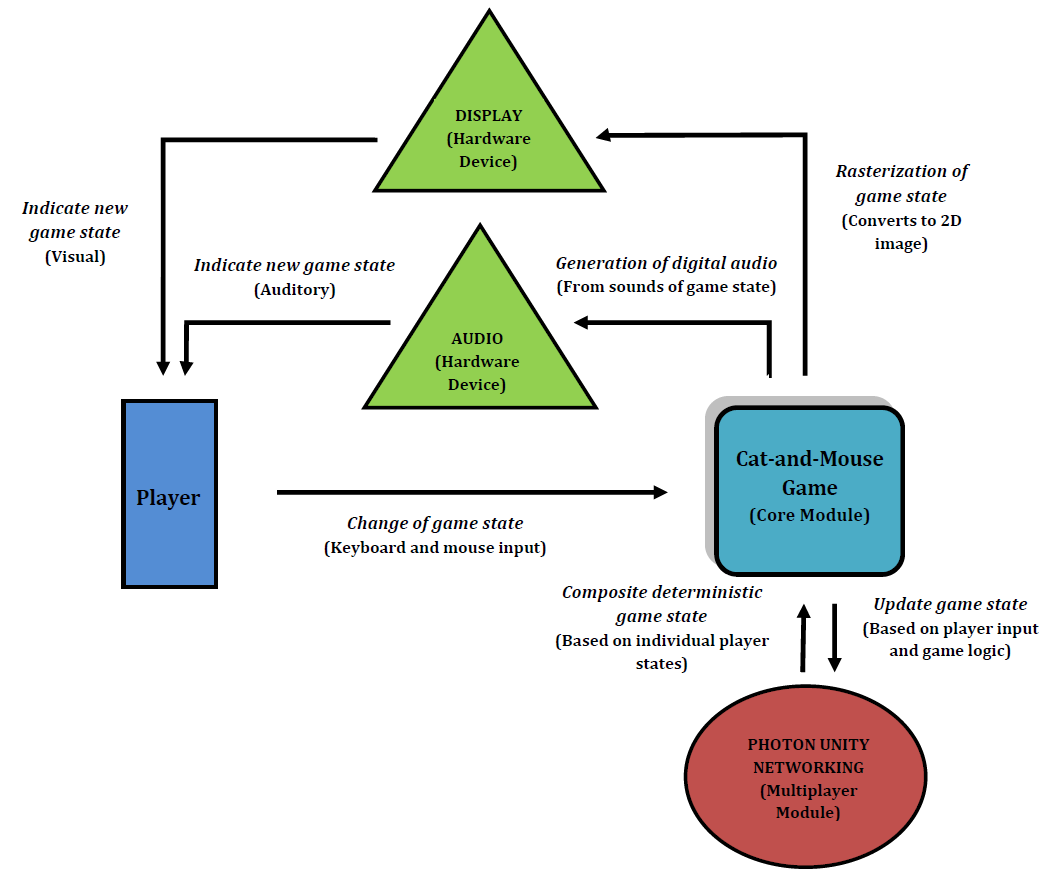
\includegraphics[width=\textwidth]{ContextDiagram.png}
\caption{Context Diagram for the Cat-and-Mouse Game}
\end{figure}
\newpage
\subsubsection{Work Partitioning}
\paragraph{}A list displaying all business events to which the game responds is indicated in \textbf{Table 2}. These 'real-world' events represent the general operations allowed in the game and indicates the action(s), if any, which should be taken.
\\
\\
\\
\begin{longtable}{| p{0.40\textwidth}p{0.20\textwidth}p{0.40\textwidth}|} 
\caption{\bf Business Event List for the Cat-and-Mouse Game}\\
\hline
{\textbf{Event Name}} & {\textbf{Input and Output}}  & {\textbf{Summary of BUC}}\\
\hline
\hline
\\
\printBusinessEvent  Player begins a new multiplayer session & \multirow{25}{0.20\textwidth}{Change of game state (in);\newline Update game state (out);\newline Composite deterministic game state (in);\newline Rasterization of game state (out);\newline Generation of digital audio (out);\newline Indicate new game state - Visual (out);\newline Indicate new game state - Auditory (out)} & A new multiplayer session is started on the server.\\
\\
\printBusinessEvent  Player enters an existing multiplayer session & & A new player is added to 'Lobby Screen' of the specified multiplayer session.\\
\\
\printBusinessEvent  Player requests to start the Tutorial & & A single player session is started on the server. The tutorial maps are loaded. The Player is assigned to a Cat or Mouse character (of their choice).\\
\\
\printBusinessEvent  Players vote on the mode of gameplay & & Each player is randomly assigned to a Team and a map is loaded. If the vote is tied, mode of gameplay is randomly selected.\\
\\
\printBusinessEvent  A single Player in a multiplayer session requests to start the match && Displays 'Player Ready' notification for that Player.\\
\\
\printBusinessEvent  All Players in a session request to start the match && All Players are assigned to a character on a Team randomly. The selected map and game mode are loaded.\\
\\
\printBusinessEvent  Player leaves the match && The  current match (if active) should continue. Players may be switched between Teams to rebalance.\\
\\
\printBusinessEvent  Player Character is moved && The Player's character is moved within the map.\\
\\
\printBusinessEvent  Player Character makes contact with the environment  && Depending on the type of environment, will affect the character's state in varying ways.\\
\\
\printBusinessEvent  Player Character is near an Item && The character is able to pick up the Item.\\
\\
\printBusinessEvent  Player Character picks up Item && The Item is transferred into character's inventory.\\
\\
\printBusinessEvent  Player Character drops Item &&  The Item is removed from character's inventory. May be picked up by other characters. \\
\\
\printBusinessEvent  Player Character uses Item in inventory && Affects the Attributes, Skills and/or Items of the character.\\
\\
\printBusinessEvent  Player Character makes contact with another Player Character from the same Team && Both players' movement is stopped.\\
\\
\printBusinessEvent  Player Character makes contact with Monster && Will drain the Health Points (HP) of the Player Character. May also inflict other effects.\\
\\
\printBusinessEvent Player Character makes contact with another Player from the opposing Team && Both Players' movement is stopped. Other effects may take place dependent on each character's respective Skills and Attributes.\\
\\
\printBusinessEvent  Player Character is near a Non-Playable Character (NPC) && Character can interact with the NPC to receive Tasks.\\
\\
\printBusinessEvent  Player Character starts Task && Players provided with specific conditions which must be furfilled.\\
\\
\printBusinessEvent  Player Character finishes Task && Players granted enhanced Attribute(s), Skill(s) and/or Item(s).\\
\\
\printBusinessEvent  Player Character attacks another Player Character from the same Team && Nothing occurs.\\
\\
\printBusinessEvent  Player Character attacks another Player Character from the opposing Team && Will drain the Health Points (HP) of the opposing Player Character (dependent on Attributes and Skills). May also inflict other effects.\\
\\
\printBusinessEvent  Player Character attacks Monster  && Drains the Health Points (HP) of the Monster. May also inflict other effects.\\
\\
\printBusinessEvent  Player Character beats Monster && Grants Player Character with enhanced Attribute(s), Skills(s) and/or Item(s).
\\
\printBusinessEvent  Player Character uses Skill && Affects the attributes of the Player Character and/or the envrionment around them (including other characters). May use up Mana Points (MP).\\
\\
\printBusinessEvent  Player Quits the game  && Player is disconnected from the server and the game returns to the "Main Menu".\\
\\
\hline
\hline
\\
%No user input Business events
\printBusinessEvent  Monster attacks Player Character & \multirow{7}{0.20\textwidth}{Update game state (out);\newline Composite deterministic game state (in);\newline Rasterization of game state (out);\newline Generation of digital audio (out);\newline Indicate new game state - Visual (out);\newline Indicate new game state - Auditory (out)} & Drains the Health Points (HP) of the Player Character. May also inflict other effects. \\
\\
\printBusinessEvent  Player Character's Health Points (HP) reaches zero &  & The Player Character will die.\\
\\
\printBusinessEvent  Player Character's Mana Points (MP) reaches zero && The Player Character will be unable to use Skills which require MP.\\
\\
\printBusinessEvent  Player Character dies && The Player Character will be returned to the "Lobby Screen".\\
\\
\printBusinessEvent  All Player Characters on a Team are beaten.  && The opposing Team is granted one Point. The current match will end. The Players will be returned to the "Lobby Screen" for the session.\\
\\
\printBusinessEvent  Player disconnects from the server && The player will be returned to the "Main Menu". An error message is displayed.\\
\\
\printBusinessEvent  All Players have left the multiplayer session && The session (and all connections) will be closed.\\
\\
\hline
\hline
\\
% No multiplayer input Business events
\printBusinessEvent  Player starts the Cat-and-Mouse Game & \multirow{3}{0.20\textwidth}{Change of game state (in);\newline  Rasterization of game state (out);\newline Generation of digital audio (out);\newline Indicate new game state - Visual (out);\newline Indicate new game state - Auditory (out)} & Displays the "Main Menu". Options to "Start New Multiplayer Session", "Start Tutorial", access "Game Options", and "Quit Game".\\
\\
\printBusinessEvent  Player selects the "Options" Menu from the Main Menu && Allows the Player to adjust various settings for the game (eg. graphics, audio, gameplay, etc).\\
\\
\printBusinessEvent  Player selects the "Quit Game" option from the Main Menu && Allows the Player to terminate the game.\\
\\
\hline
\hline
\end{longtable}
\newpage
\subsubsection{Individual Product Use Cases}
\paragraph{}Ideally, the user would receive the game from an online source such as a game distribution platform such as Steam, where they would download the game and install it. Individually, the game cannot be played but when they join the game's online rooms they will be able to find other players also looking for games to join. The user will then be able to play the game with other people online. 
\subsection{Functional Requirements}
\textbf{Requirement 1:}  The Cat-and-Mouse Game should allow players to adjust in-game options (such as graphics, audio, the UI and gameplay settings) to suit their preferred experience and hardware.\\
\textbf{Rationale:}  This will allow for the product to be accessible to a broader audience as well as a wider variety of hardware.\\
\textbf{Fit criterion:}  Players have the ability to set the graphics fidelity in-game to match their computer's capabilities, toggle audio (background music, sound effects), customise input controls, as well as personalise the placement of various elements of the User Interface to their liking.\\
\\\\
\textbf{Requirement 2:}  The Cat-and-Mouse Game should allow players to join a Multiplayer Hub located on a server wherein they can interact and communicate with other players.\\
\textbf{Rationale:}  This will allow Players to meet and greet their teammates for the upcoming Match and foster a sense of camaraderie. Players will also have the chance to decide together on a game mode and discuss strategy during the match. \\
\textbf{Fit criterion:}  Players are able to connect successfully to the game server and communicate via text or voice with their teammates both in the Multiplayer Hub and while a match is in progress.\\
\\\\
\textbf{Requirement 3:}  The Cat-and-Mouse Game should allow players to collaboratively customise various aspects of the Match to suit their preferences.\\
\textbf{Rationale:}  To appeal to a wide audience, players should have the freedom to adapt their gameplay experience according to their interests, skill level and play style.\\
\textbf{Fit criterion:}  Players are able to chose from a variety of in-game modes, maps and difficulty settings. Players should be able to agree on these settings through a vote-based system.\\
\\\\
\textbf{Requirement 4:}  The Cat-and-Mouse Game should randomly assign Players to play on either the 'Cat' or 'Mouse' team for every Match.\\
\textbf{Rationale:}  This introduces a competitive element to the game, as well as fosters a sense of camaraderie, to encourage effective teamwork and collaboration between members fighting for the same cause. \\
\textbf{Fit criterion:}  Players are able to chose from a variety of in-game modes, maps and difficulty settings. Players should be able to agree on these settings through a vote-based system.\\
\\\\
\textbf{Requirement 5:}  The Cat-and-Mouse Game should allow players to see and interact with each other through avatars in real-time to complete tasks and obectives within a virtual maze. \\
\textbf{Rationale:}  This aspect enables key collaborative elements around which the core mechanics and gameplay have been designed.\\
\textbf{Fit criterion:}  Individuals are able to see the position and status of, as well as interact with the virtual environment simultaneously with the other players participating in the match.\\
\\\\
\textbf{Requirement 6:}  The Cat-and-Mouse Game should allow players to move their characters around the map as the environment allows. \\
\textbf{Rationale:}  Ensuring freedom of movement encourages players to be adventurous and creative in their interactions with not only the game objectives, but other fellow participants as well.\\
\textbf{Fit criterion:}  Individuals are able to move to any point in the map without going through walls or solid objects.\\
\\\\
\textbf{Requirement 7:}  The Cat-and-Mouse Game should allow players to attack and deal damage to the corresponding players on the opposing team. \\
\textbf{Rationale:}  This allows for game progression, and encourages team cooperation by introducing a survival element to the gameplay.\\
\textbf{Fit criterion:}  Players are able to wield various attack and defensive skills to cause damage to a player on the opposing team. The ability to utilise  skills is regulated by a Mana Indicator, which must be kept filled. Remaining Health is also indicated and upon reaching a certain level, the player "dies" and is (temporarily) unable to participate further in the match.\\
\\\\
\textbf{Requirement 8:}  The Cat-and-Mouse Game should allow teams to gain points through acomplishing certain in-game tasks or objectives, depending on the selected game mode. Game modes include: capture the flag, escape the maze, and team deathmatch. killing opponents, capturing the flag, and killing cpu controlled monsters all give points.\\
\textbf{Rationale:}  This allows for game progression, and a the competitive element encourages greater team cohesion in order to get ahead.\\
\textbf{Fit criterion:}  Each team is granted points for accomplishing certain objectives over the course of a match. Dependent on the mode and parameters of the match, the game is considered "won" either when a Team attains the highest number of points after a certain period of time, a special condition has been fulfilled (e.g. capture the flag), or all members of the opposing Team have been eliminated.  \\
\\\\
\textbf{Requirement 9:}  The Cat-and-Mouse Game should ensure that all players start on an even level playing field, so that there is a lower barrier of entry for new and casual players.\\
\textbf{Rationale:}  The social nature of the game and strong focus of the game around teamwork and cooperation is such that the need for such skills to succeed should not be mitigated by the sheer amount of time spent in-game.\\
\textbf{Fit criterion:}  Limited or no game state data is retained upon the termination of a multiplayer session. When starting a new game, previous player performance and accomplishments do not impact the skills or abilities which are granted to a player. Although both the 'Cat' and 'Mouse' Teams host varying Skills and Attributes, the game mechanic will be balanced so that neither team has a predetermined advantage over the other.\\
\\\\
\textbf{Requirement 10:}  The Cat-and-Mouse Game should allow for opportunities for Players to enhance their Skills and Attributes through various in game interactions, such as by completing quests, defeating Monsters and collecting Items and Consumerables.   \\
\textbf{Rationale:}  The ability (and indeed, necessity) for a Player to work their way up from baseline in every session motivates individuals to fully explore all the possbilities which are present in every situation. Thus, all participants will be fully engaged in the game experience, and newcomers to the game will not be at a disadvantage in term of enjoyment (e.g. in terms of more 'experienced' players using the same skills over and over again in every match).\\
\textbf{Fit criterion:}  All Players are able and encouraged to interact with the game envrionment (and other players) in new and innovative ways in every match, and a variety of different paths to the same goal will provide for high replay value for even the most seasoned players.\\
\\\\
\section{Non-Functional Requirements}
\subsection{Look and Feel Requirements}
\subsubsection{Appearance Requirements}
\paragraph{}The game's interface shall be attractive to audiences of all ages and customers should be able to easily and quickly use the interface as it will be as intuitive as possible. We will use darker colours for the most part, avoiding flashy or warm colours in favour of colder colours to match the labyrinth theme and to help create a sense of tension.  
\subsubsection{Style Requirements}
\paragraph{}We want this game to appear simple and intuitive, so that it does not intimidate certain age groups. However, it will have a mature look to it and a western art style, and together they will create a intense, dungeon-like feel. The players should feel a light sense of tension when playing, the Cat because he wants to find the Mice as soon as possible and the Mice because they do not want to be found.  
\subsection{Usability and Humanity Requirements}
\subsubsection{Ease of Use Requirements}
\paragraph{}The product will be easy to use for users of all ages, requiring basic English skills and use of a computer mouse and keyboard. The user should be able to learn the basics of the game very easily, namely the controls, core mechanics, and the objective of the game with merely going through a quick tutorial. All players who successfully complete the tutorial should be able to understand the basic components of the game. 
\subsubsection{Personalization and Internalionalization Requirements}
\paragraph{}The basic controls will be customizable, allowing the user to change certain hotkeys to whatever they please. The interface will be semi-customizable, allowing the user to move or resize items to their preference. 
\paragraph{}The first release of the product will only support English, but it will be very basic English that even individuals not fluent in English will be able to understand. Upon further development, we may include language packs such as French or Chinese. 
\subsubsection{Learning Requirements}
\paragraph{}Even though the game will be designed to be easy to learn, and easy to get a basic feel of the game, it will be very hard to master. Playing this game at the highest level will require the user to memorize the most efficient paths or abilties, and make very few errors in terms of gameplay. The game should be difficult enough to inspire motivation to improve, but also easy enough to avoid discouraging users from playing. A benchmark will be such that a new user will have a general feel of the game after going through the tutorial, but becoming a master at the game will take hundreds of hours of gameplay. The game should have a lasting impression on the users in terms of fun and desire to improve, and make them want to come back and play again. 
\subsubsection{Understandability and Politeness Requirements}
\paragraph{}Since the product is a video game, there will be concepts that are foreign to non video game players. However, the basic concept of the game is designed around the game "cat and mouse" which most people should be familiar with; a game where the cats try to catch the mice. A tutorial will be included in the game, and will be written in a way that is easy to understand for anyone, avoiding difficult concepts or jargon when possible, and explaining them in detail when required. 
\subsubsection{Accessibility Requirements}
\paragraph{}As a video game, the physical aspect cannot be easily substituted as the user will always be required to control their character using a keyboard and mouse, or a modified controller. The visual aspect also cannot be replaced as the user is required to be able to see everything that is going on in game, so fully blind individuals will unfortunately be unable to use this product. However, we can provide options for the colorblind by changing the in game colors to suit their needs. To suit the needs of the deaf, we can have subtitles of annotations for them to read. 
\subsection{Performance Requirements}
\paragraph{}We hope to target players of all demographics, and we hope that they will be able to enjoy our game even if they do not have the latest computer systems. We will thus design our game to run smoothly on older computers as well as newer models.
\subsubsection{Speed and Latency Requirements}
\paragraph{}As the game operates at a real time level and is also multiplayer, we want each player to constantly have updates on the current game state. This would require information packets to be sent to each player multiple times every second, and each group of packets will contain information such as other the movements or actions of other players. The users will therefore be required to have a minimum internet connection speed of 1 Mbps. 
\paragraph{}Latency is also an important issue to consider in a real time game such as the one we are developing. Players need to be able to react immediately to what is going on in the game, so their latency should be as low as possible. We will aim to limit each player's ping to 100 ms or less, as any more than this causes an obvious delay between the user's physical actions and their characters actions. 
\subsubsection{Safety-Critical Requirements}
\paragraph{}The game will not have any extremely flashy effects that can cause seizures for certain individuals. 
\subsubsection{Precision or Accuracy Requirements}
\paragraph{}N/A.
\subsubsection{Reliability and Availability Requirements}
\paragraph{}The server that a user hosts should not fail until said user closes it themselves. If the user leaves the game but does not close the server, then it should persist. The game itself should also not crash under any circumstance.
\subsubsection{Robustness or Fault-Tolerance Requirements}
\paragraph{}If a server is shut down unexpectedly, the game should kick players and display an error message to let them known what has happened. Any other unexpected errors should also display a message to the clients. If any player leaves the game, the game should continue as usual and switch a player to the other team if it is unbalanced.  
\subsubsection{Capacity Requirements}
\paragraph{}Each game instance will host up to four players at a time, and information for each player will need to be stored on the server at any given time. For each user, the game will need to receive and hold data on each of the other three players as well as the current game state. 
\subsubsection{Scalability or Extensibility Requirements}
\paragraph{}If the game increases in popularity then our servers will need to be upgraded to handle the increased traffic. The game itself will also be able to handle frequent patches to fix bugs or add new features. 
\subsubsection{Longevity Requirements}
\paragraph{}As a computer video game, the expected lifetime of the product is as long as the user is interested in playing. A typical user can be expected to play for 1-2 hours, however if frequent updates are made to the game and the user constantly finds it fun, then the game's lifetime can be much longer. 
\subsection{Operational and Environmental Requirements}
\subsubsection{Expected Physical Environment}
\paragraph{}N/A.
\subsubsection{Requirements for Interfacing with Adjacent Systems}
\paragraph{}This game should work with Windows 7, 8, 8.1 and 10. It should also work with DirectX 11 and DirectX 9 as those are the graphics API that we will be using with Unity. 
\subsubsection{Productization Requirements}
\paragraph{}This product will require users to have either DirectX 9 or DirectX 11 installed. The product will be distributed as a ZIP file, all users need to do is unzip it.
\subsubsection{Release Requirements}
\paragraph{}Ideally the game will be released on a game platform such as Steam, which allows users to receive updates with ease. However the first versions of the game will be released as a downloadable bundle where the user will have to download and install manually, then open the game by running the executable files. 
\subsection{Maintainability and Support Requirements}
\subsubsection{Maintenance Requirements}
\paragraph{}Patches and updates will be released as the creators see fit, in order to address bugs in the game, issues with balancing, or to release new game content. 
\subsubsection{Supportability Requirements}
\paragraph{}The game will require minimal support, however if the user encounters issues with the game then they can contact the creators directly to look for a fix. 
\subsubsection{Adaptability Requirements}
\paragraph{}Currently, we do not plan on porting the product no other platforms or environments.
\subsection{Security Requirements}
\subsubsection{Access Requirements}
\paragraph{}The users will only be able to access the main game and the options that we see fit. The source code and server code will be hidden and restricted from the user. 
\subsubsection{Integrity Requirements}
\paragraph{}Serious damage can be caused if an outsider gains access to the source code, so steps will be taken to prevent unauthorized access. Hacking into the servers can also cause issues with cheating and players gaining unfair advantages, so steps will also be taken to stop outside attacks. 
\subsubsection{Privacy Requirements}
\paragraph{}This game will not have private information stored. The only information a user will have is their username, which will be stored on the client's machine.
\subsubsection{Audit Requirements}
\paragraph{}N/A.
\subsubsection{Immunity Requirements}
\paragraph{}Users having anti-virus software should be sufficient for protection against unauthorized programs like viruses.
\subsection{Cultural Requirements}
\paragraph{}The product will not have anything offensive or sensitive, culturally or religiously. The game will be in english and is not intended for a market outside of the US and Canada.
\subsection{Legal Requirements}
\subsubsection{Compliance Requirements}
\paragraph{}All of our assets and code will be created by ourselves or royalty free.
\subsubsection{Standards Requirements}
\paragraph{}N/A.
\subsection{Health and Safety Requirements}
This section is not in the original Volere template.
\paragraph{}We do not want our game to use flashing imagery and effects that can potentially cause health issues such as seizures. This includes effects such as the game frequently flashing bright colors at the user, and use of certain patterns which can trigger an seizure in the affected demographics.
\section{Project Issues}
\subsection{Open Issues}
\begin{itemize}
    \item Finding a good balance to the game is an issue. Because teams are asymmetrical (there is only 1 cat, while there is 3 mice), and each team has different abilities, it's hard to gauge how fair it is for one team which can affect how much fun the players have playing this game. 
    \item Still need to think of an algorithm for map generation that makes the maps enjoyable to play on. 
\end{itemize}
\subsection{Off-the-Shelf Solutions}
\subsubsection{Ready-Made Products}
\paragraph{}N/A
\subsubsection{Reusable Components}
\paragraph{}N/A
\subsubsection{Products That Can Be Copied}
\paragraph{}There are asymmetrical player versus player games currently on the market, which if we could legally copy them, it could help with our game's potential balancing issue. A game that comes to mind is Evolve, which has one team being composed of a single player playing as a monster, and four hunters as the other team. Similar to ours, the teams have their own unique abilities and skillset. 
\subsection{New Problems}
\subsubsection{Effects on the Current Environment}
\paragraph{}N/A
\subsubsection{Effects on the Installed Systems}
\paragraph{}N/A
\subsubsection{Potential User Problems}
\paragraph{}N/A
\subsubsection{Limitations in the Anticipated Implementation Environment That May Inhibit the New Product}
\paragraph{}The game might not run optimally depending on the hardware a user uses to run it. 
\subsubsection{Follow-Up Problems}
\paragraph{}N/A
\subsection{Tasks}
\subsubsection{Project Planning}
\begin{itemize}
    \item Produce sufficient and necessary documents such as requirement document, user guide, etc. 
    \item Acquire necessary knowledge about tools we are using, and to familiarize ourselves with them. 
    \item Develop a playable prototype of the game without all the features yet. 
    \item Add on to the the prototype.
\end{itemize}
\subsubsection{Planning of the Development Phases}
\begin{itemize}
    \item Basic movement/controls of the characters.
    \item Map generation algorithm.
    \item Networking so multiplayer works.
    \item Creating the game's interfaces such as menus.
    \item Adding abilities and objectives to the game.
    \item Re-balancing the game after acquiring appropriate feedback from testers.
    \item Adding graphics and sounds that are not placeholders to polish the game's aesthetics.
\end{itemize}
\subsection{Migration to the New Product}
\subsubsection{Requirements for Migration to the New Product}
\paragraph{}N/A
\subsubsection{Data That Has to Be Modified of Translated for the New System}
\paragraph{}N/A
\subsection{Risks}
\begin{itemize}
    \item Certain abilities might be badly balanced, and thus make it unfair for one team.
    \item Procedurally generated maps using algorithms might affect balance of the game. 
    \item Might not be able to find enough play testers to give satisfying feedback.
    \item Could run into trouble with networking and making it playable online.
    \item Time could be badly managed, and will need to cut down on features.
\end{itemize}
\subsection{Costs}
\paragraph{}There will be a time cost of 7 months for development of the game, but will cost no money as all tools used are free.
\subsection{User Documentation and Training}
\subsubsection{User Documentation Requirements}
\paragraph{}We will provide a User Documentation, as it is required as part of our capstone. There will also be a tutorial in game that informs players about the rules and how to play the game. This tutorial will cover topics such as joining a game, joining a team, movements, and objectives of the game. 
\subsubsection{Training Requirements}
\paragraph{}The game will require users to know basic English in order to go through the tutorial and play the game.
\subsection{Waiting Room}
\paragraph{}A requirement that might be done after the initial release of the product is an installation wizard. For now we think it is best to stick with an executable file for the game. Using an installation wizard also gives us the option to use more external dependencies, and thus more features if needed. any further requirements that might be added will be listed here as the document is revised.
\subsection{Ideas for Solutions}
\paragraph{}Currently, we do not have any ideas for solutions. This might change as we update this document.
\bibliographystyle{plainnat}
\bibliography{SRS}
\end{document}